\subsection{Data description}
The training data $imgs$ contains 8545 color images of size 105x43. From every image a HOG descriptor 26x10x36 was extracted and converted into a vector of total length 9360. All of these descriptors form the training data that we will work on. 

\noindent We notice that there are 7308 images without presence of people (negative images) and 1237 with (positive images). Fig\ref{fig:starting_images} presents a typical example from each category along with the corresponding feature descriptor.

\noindent Our task is to train various classifiers, so that we will be able to detect the presence of people in new images. For this purpose we evaluate five classifiers, measuring the accuracy of their estimations using Receiver Operating Characteristics (ROC) curves.

\begin{figure}[h]
  \centering
  \begin{subfigure}[b]{0.45\textwidth}
   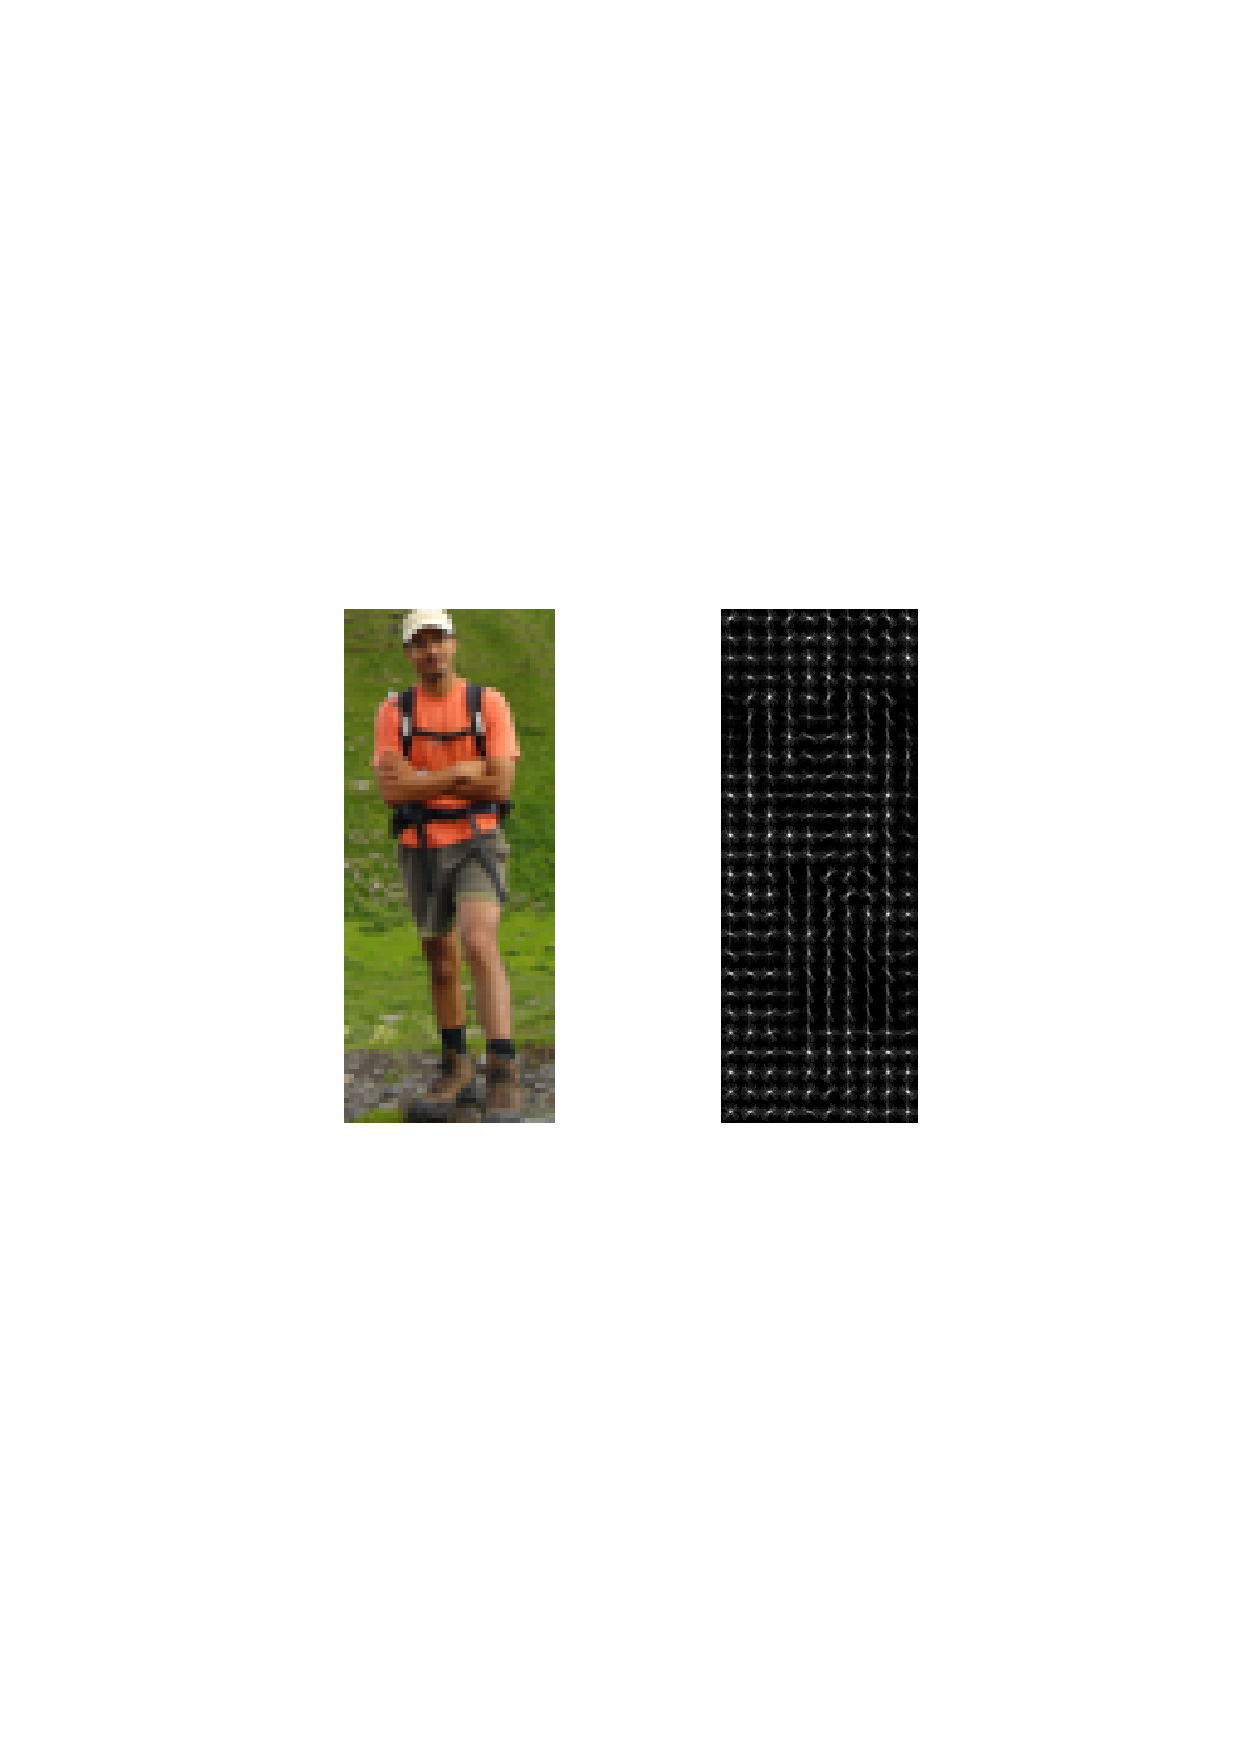
\includegraphics[width=\textwidth]{figures/positive_image.pdf}
    \caption{Positive image.}
  \end{subfigure}
  \begin{subfigure}[b]{0.45\textwidth}
    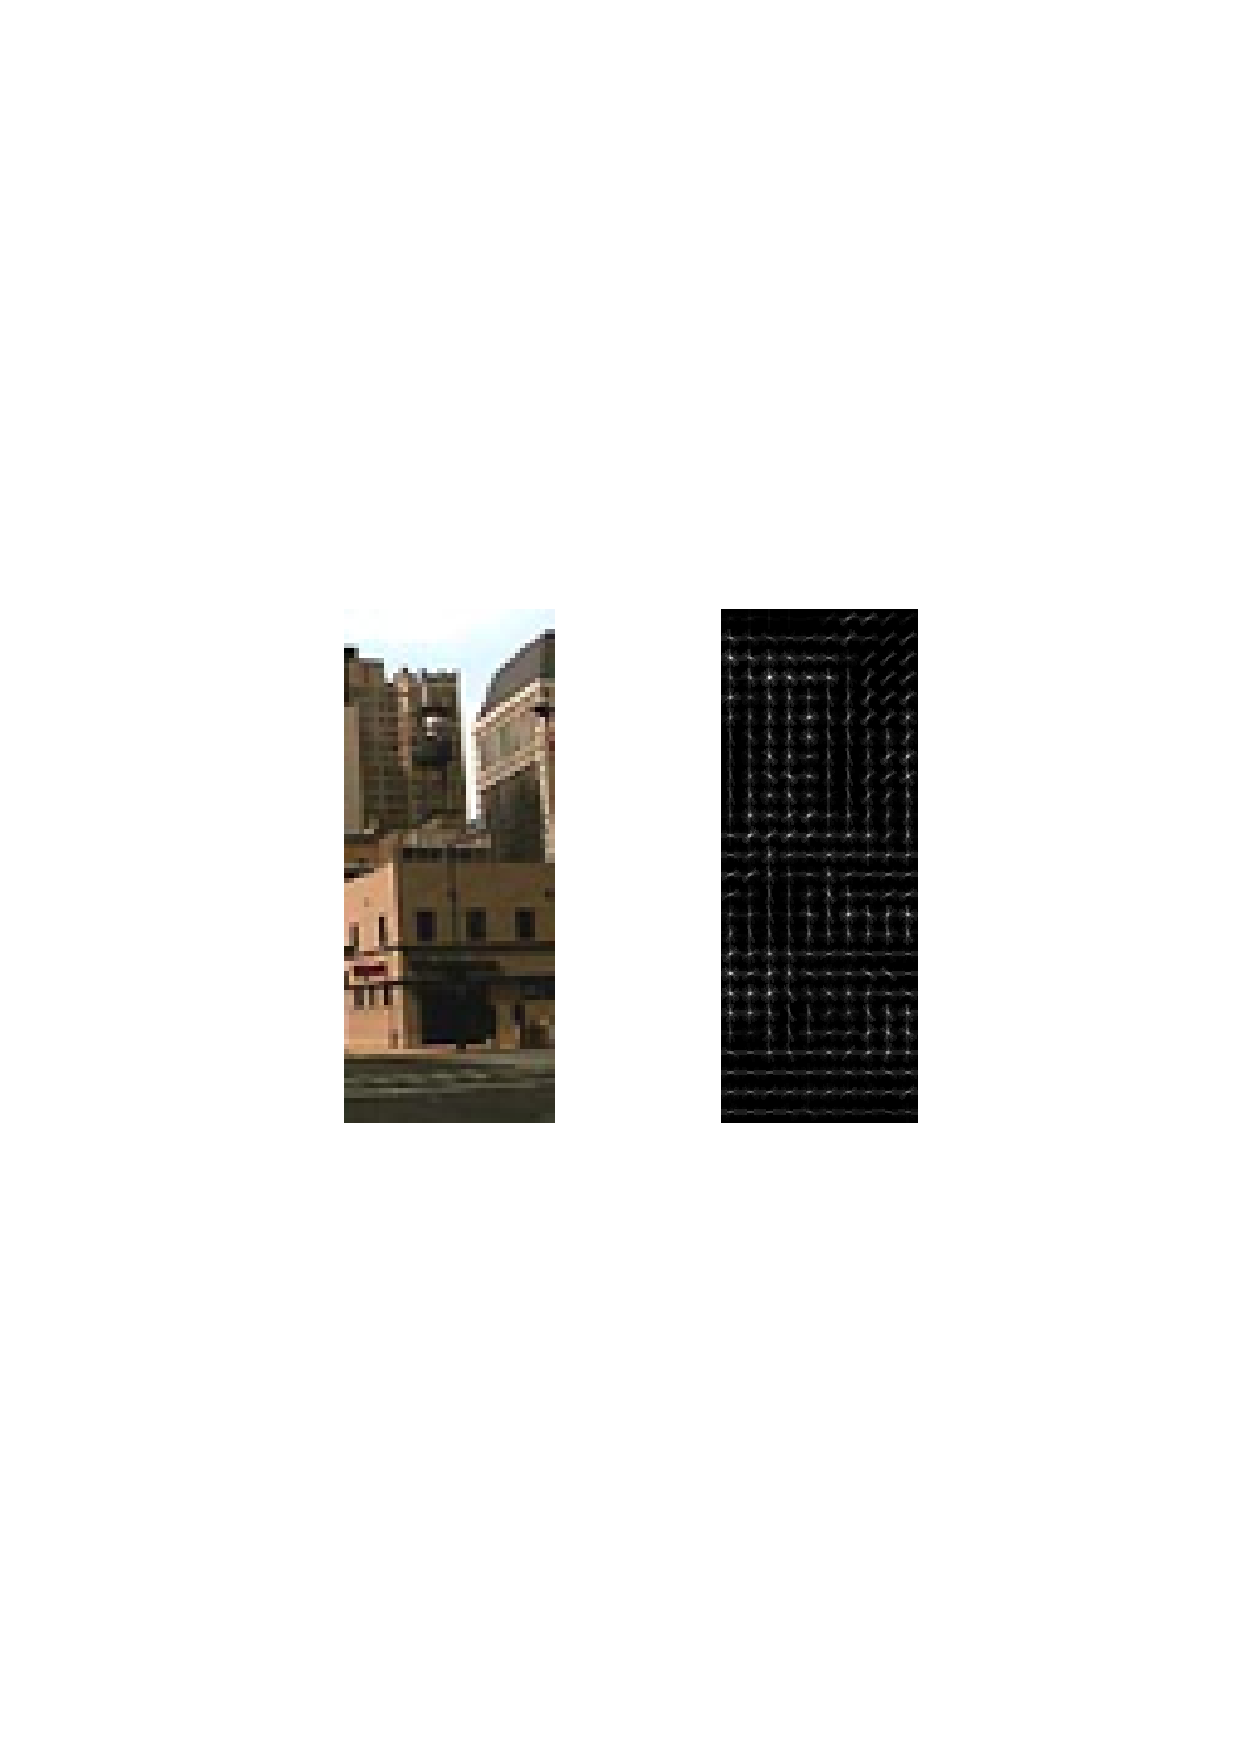
\includegraphics[width=\textwidth]{figures/negative_image.pdf}
    \caption{Negative image.}
  \end{subfigure}
  \caption{Examples of positive and negative images and their corresponding feature descriptors.}
  \label{fig:starting_images}
\end{figure}

\subsection{Data preprocessing}
\noindent We assume that there are no outliers, since the images are manually annotated. We work on the extracted features so we normalize the 9360 dim vectors to have  0 mean and standard deviation 1.

For all the methods presented below we used 5 fold cross validation.

\noindent The methods that we compare are the naive Bayes classifier, the logistic and penalized logistic regresion, the Support Vector Machine (SVM), the K-NN classifier, and the Neural Network classifiers. All of them are compared also with the random guess of the class in a later subsection of the report.

\noindent We note that before the experiments we tried using PCA for reducing the dimensionality of the feature descriptors. The reduction in dimensionality was minimal but at a huge computational cost so we decided to drop it.
\textcolor{red}{TODO ask vasilis what was the reduction}

\subsection{Naive Bayes classifier}
\noindent In this part we tried to fit a simple Bayes classifier to our data. For this, we made the assumption that the data is normally distributed and the estimates of the prior probabilities can be estimated empirically from the relative frequencies of the classes in training.

\noindent The results from the K-fold validation were not very satisfying, since the average TPR was very low (0.031). The reason that may be hidden behind that are the strong assumptions that we made in order to fit this model. Naive Bayes model assumes that the data that will process every time follow a specific distribution (in our case Gaussian), but also that the value of a particular feature is unrelated to the presence or absence of any other feature, given the variable of the class. In our case, this is possibly wrong, so the classifier cannot fit a appropriate model.

\subsection{Logistic and Penalized Logistic Regression}
\noindent Our purpose in this part was to fit the logistic regression and its penalized version to our data. The value for the parameter $\alpha$ that we used was $10^{-2}$, since all of the values close to this performed well enough for our experiments. Moreover, regarding the value for $\lambda$ in case of the penalized logistic regression, we have to mention that all of the values that were used performed the same. This is the reason that both of the method give the same results, with average TPR equal to 0.754.

\noindent During penalization the idea is to avoid the overfitting by imposing penalty on large fluctuations of the model parameters and reduce the influence of the outliers to our model. This is possibly the reason that both models perform equivalently. The data, as we mentioned before, do not have outliers and the fluctuations at the model parameters are avoided by the nature of our data.

\subsection{Support Vector Machines}
\noindent For the certain part of the experiment we used the LIBSVM 3.20 toolbox that includes SVM using various kernels. In our case, we performed analysis and K-fold validation on linear-kernel SVM, polynomial-kernel SVM with degrees 2 and 3, real-basis-kernel SVM and sigmoid-kernel SVM. In all of the cases we used the scores that were given by the program to compute the TPR and the FPR. A comparison of the various cases is given in Figure \ref{fig:SVM}.

\noindent As we can observe radial-basis-kernel SVM have significantly good performance. A fact that can be seen not only by the average TPR, which is equal to 0.893, but also observing the whole range of the FPR, where the classifier gives better results than all of the other SVM cases. The second best in performance is the polynomial SVM with degree 2, which has very similar results with the RBF case for FPR greater than $2 10e{-3}$. The rest of the classifier perform well for FPR greater than $2 10e{-2}$, with the exception of the linear case, which has quite good results for lower rates, too.

\noindent Moreover, in Table \ref{table:SVM_success} we present the average percentage of the successful classifications that were made during the K-fold validation, as they are given by the program.

\begin{table}[h]
  \centering
  \begin{tabular}{ | c | c | c | c | c | c |}
  \hline
  SVM kernel & Linear & Quadratic & Cubic & RBF & Sigmoid \\ \hline
  Average success rate (\%) & 94.81 & 97.22 & 91.45 & 98.43 & 84.68 \\ \hline
  \end{tabular}
  \captionof{table}{Average percentage for the success rate for the various kernels of the SVM classifier, as they are given by the program of the LIBSVM 3.20 toolbox.}
  \label{table:SVM_success}
\end{table}
    
\subsection{K-NN classifier}
\noindent Using the K-NN classifier the most important parameter that we have to specify is the number of the neighbouring samples that will be used as a reference for the method so it will decide for any given sample the class that it belongs to. For our experiments we used a ready function, which we modified a lot in order to compute and give in output the scores of the prediction, except of the class labels. We varied the number of neighbours used among 5, 9, 15, 19 and 25. In addition, the euclidean distances were used as the way to specify the distances among the neighbouring samples.

\noindent Figure \ref{fig:K_NN} presents the resulting ROC curves that were created using the scores got from the K-fold validation process. There we observe that all of the classifiers show very good performance, especially, for FPR greater than $10^{-3}$. Only the 9-NN classifier seems to perform a bit worse for FPR between $10^{-4}$ and $10^{-3}$. These observations can be explained by the distribution of the data, where most probably they are distributed in the N-dimensional (N = 9360) space with such a way that their neighbours can specify, with high probability, the class that they belong to.

\begin{figure}[h]
  \centering
  \begin{subfigure}[b]{0.49\textwidth}
   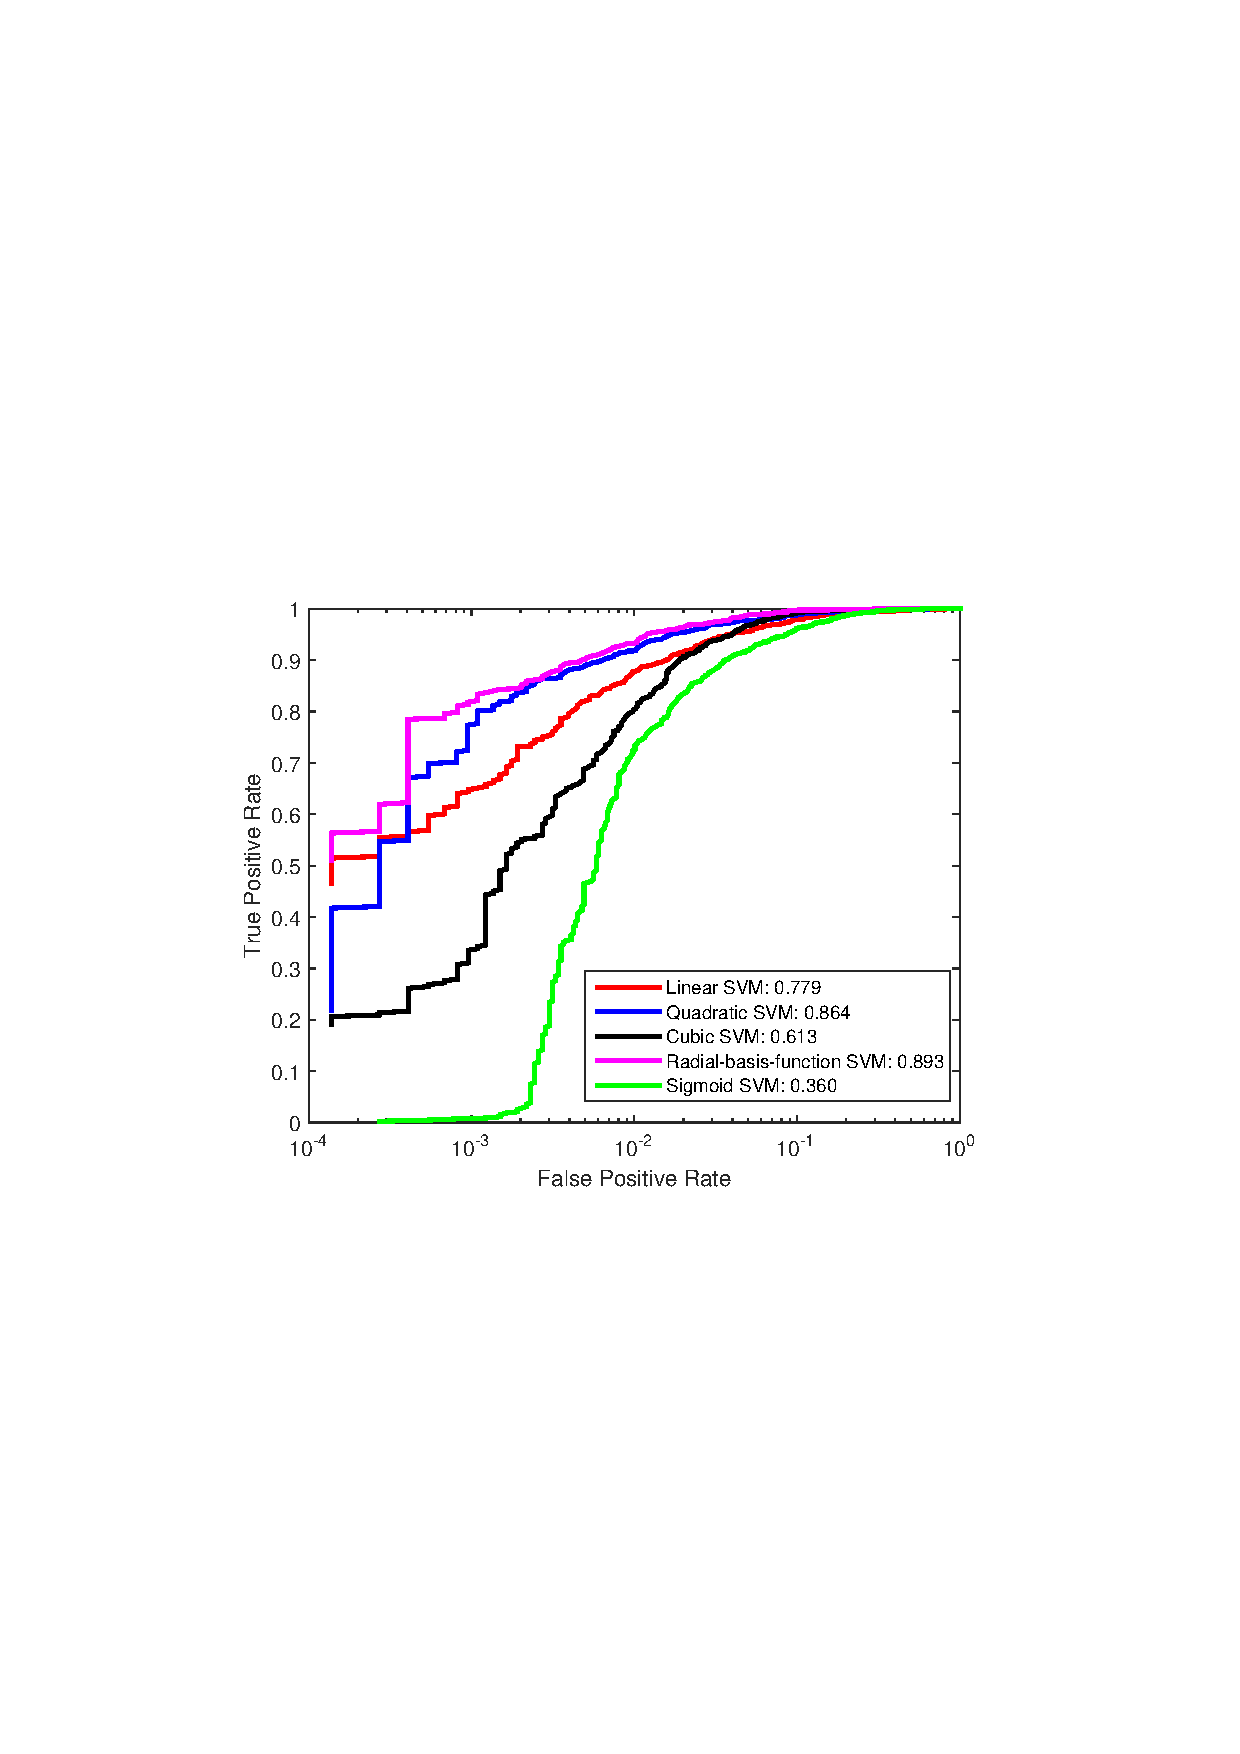
\includegraphics[width=\textwidth]{figures/SVM.pdf}
    \caption{}
    \label{fig:SVM}
  \end{subfigure}
  \begin{subfigure}[b]{0.49\textwidth}
    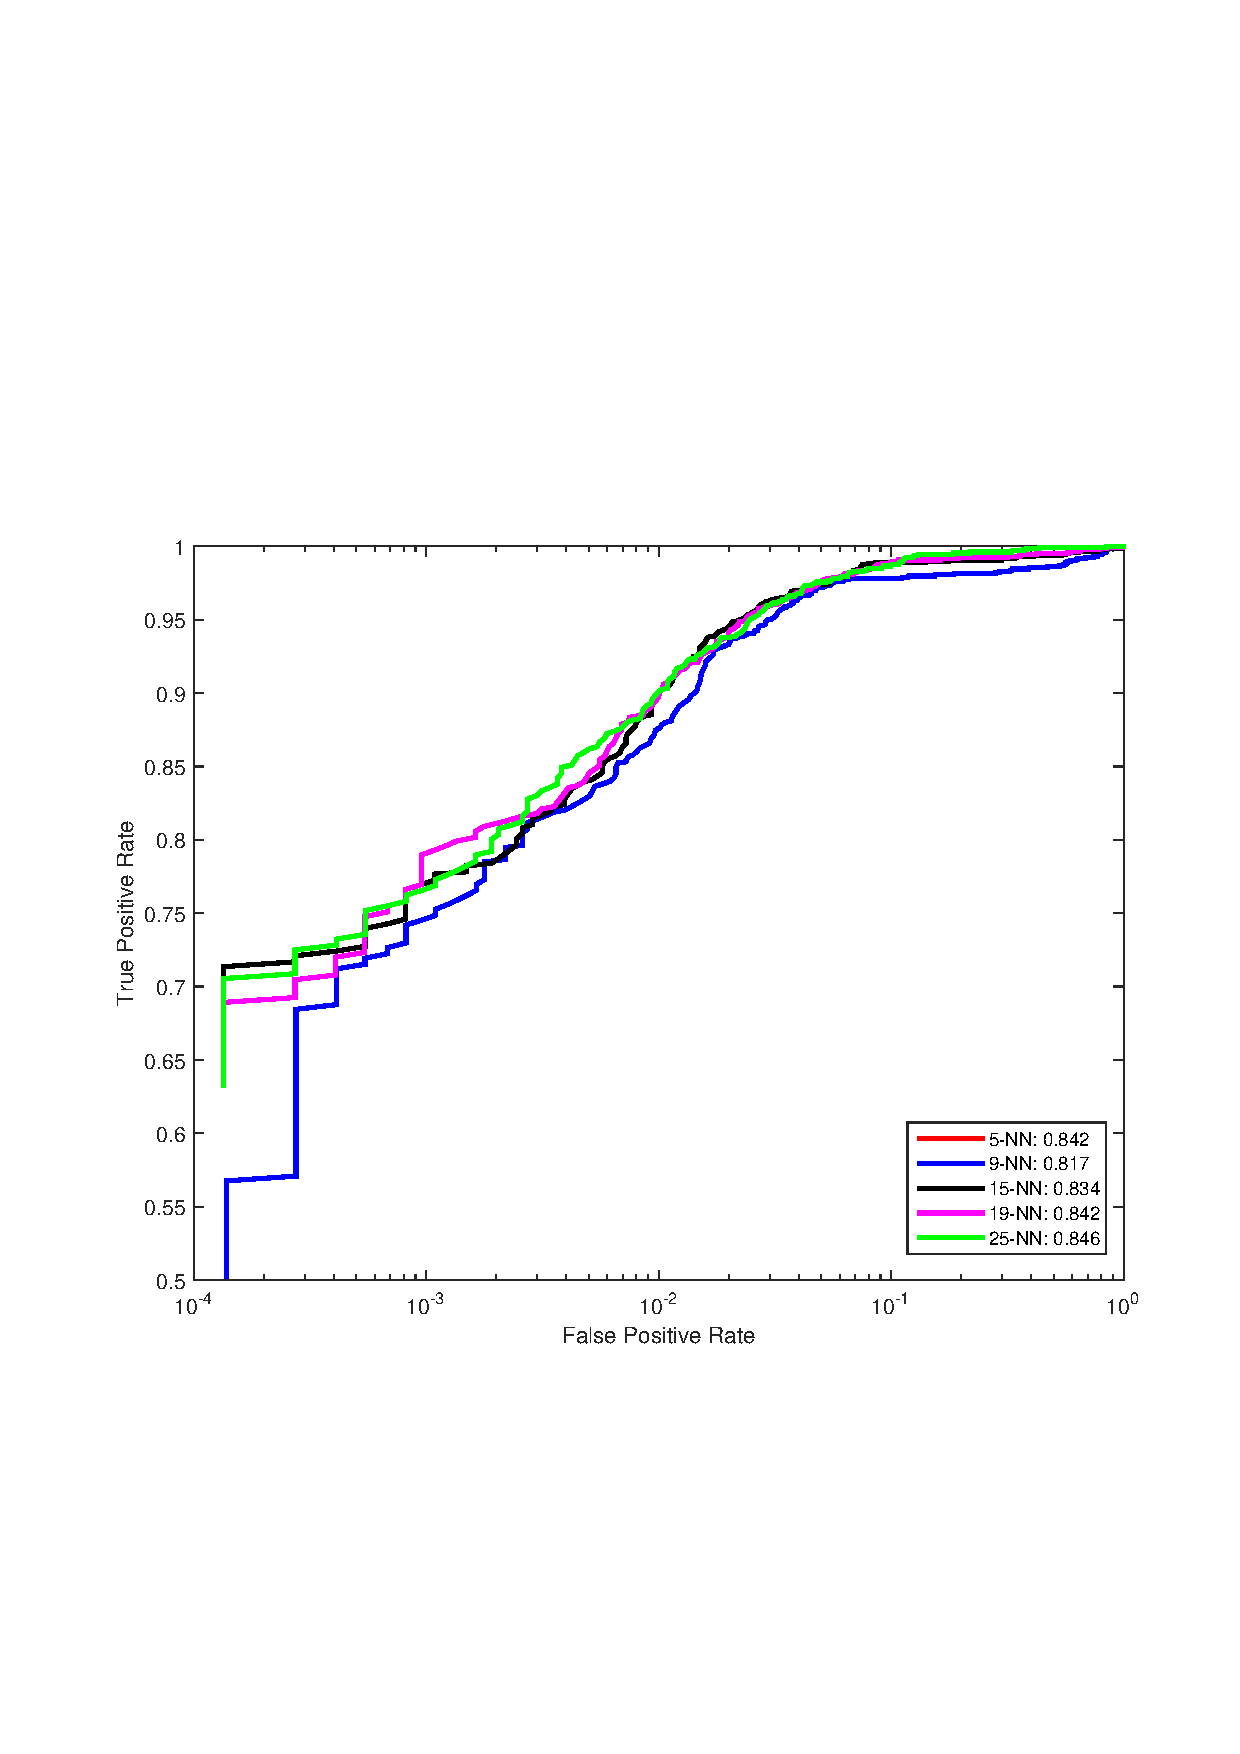
\includegraphics[width=\textwidth]{figures/K_NN.pdf}
    \caption{}
    \label{fig:K_NN}
  \end{subfigure}
  \caption{ROC curves created using: (a) SVM with various kernel types (linear, quadratic, cubic, real-basis-function, sigmoid), (b) K-NN classifier for various number of neighbours for the computations (5, 9, 15, 19, 25).}
\end{figure}

\subsection{Neural Network}
\subsection{Convolutional Neural Network}
\subsection{Comparison}